\subsection{Feature and model identity}
A deployment contract includes feature names, ordering, admissible numerical domains and every fitted preprocessing parameter. Logistic regression requires its original coefficients and intercept; the random forest requires original split thresholds, topology and leaf distributions. K-Means requires training imputation, signed-log transformation, scaling and centers. Applying a convenient replacement transform would silently define a different model. Portable parameters are therefore verified against their archived source identities and independent Spark outputs before being accepted for interactive use.

Blank permitted inputs use training medians rather than statistics computed from a user's batch. Values outside the declared finite nonnegative range are diagnosed, and invalid rows remain distinguishable in exported results. This matters for reproducibility: silently dropping rows would change output counts, while silently coercing malformed values could create apparently valid predictions. The bounded upload interface is an engineering demonstration; it does not supply missing network context or validate measurements from arbitrary extractors.

\subsection{Fairness of the external comparison}
Column-name overlap is only a starting point for cross-dataset harmonization. Units, extraction windows, aggregation semantics and upstream filtering can differ. The three common features are explicitly conditional, and the external comparison excludes unsupported exact archived transfer. The source-only and target-trained models have different fitting populations and are reported separately. Neither the target chronological nor grouped result should be relabeled as source-only transfer.

Collision exclusions also affect the estimand. Excluding predictor collisions reduces a direct role-overlap route, but changes the retained population; it does not make two capture systems identical. The chronological and grouped test counts and exclusions are consequently preserved independently. Grouped hash sampling is approximately one seventh of the relevant population rather than an independent ten-percent sample within every role. Sample inclusion and cross-role purging are documented so that a reproduction does not silently create a different experiment.

\subsection{Operating budgets and adaptive selection}
A low false-positive budget constrains a detector's threshold on permitted validation data. It is not a guarantee that future benign captures have the same score distribution. The external source RF result illustrates the distinction: a threshold accepted under source validation can exceed that ceiling on a new source. Similarly, a high target ranking score can coexist with low calibrated recall when the selected budget requires a high threshold. Reporting a fixed 0.5 comparison is informative only when it is clearly separated from the predeclared calibrated result.

Adaptive policies add a second selection problem. A candidate must be trained on allowed released labels and accepted using the policy's history and budget, with activation restricted to a later prediction window. Reporting only the best candidate after observing all future errors would violate this ordering. Incumbent retention, cooldown and failed promotion are therefore part of the measured policy behavior. More candidate fitting is not intrinsically better when false positives, delayed labels or unstable calibration dominate the trade-off.

\subsection{Independent checks and scope accounting}
Numerical verification is layered. Source audits establish counts and eligibility; role receipts establish disjointness and purges; scoring receipts attach model and threshold identities; selected pattern rules are independently recounted; explanation receipts check reconstruction; and portable probes compare the implementation against Spark without retraining. These checks address different possible defects. Passing a portable parity check cannot repair poor temporal generalization, and passing a split check cannot establish external feature compatibility.

Experimental scope counts are likewise kept separate. Warm-up runs are not additional measured replicates. Synthetic policy configurations are not independent historical populations. An exported subset is not the complete set mined by FP-growth. The final evidence matrix records accepted phase checkpoints, while the master table attaches metric selectors and source hashes to key claims. This permits a reviewer to assess both a numerical assertion and the population to which it applies without relying on an unqualified dashboard headline.

\begin{figure}[t]\centering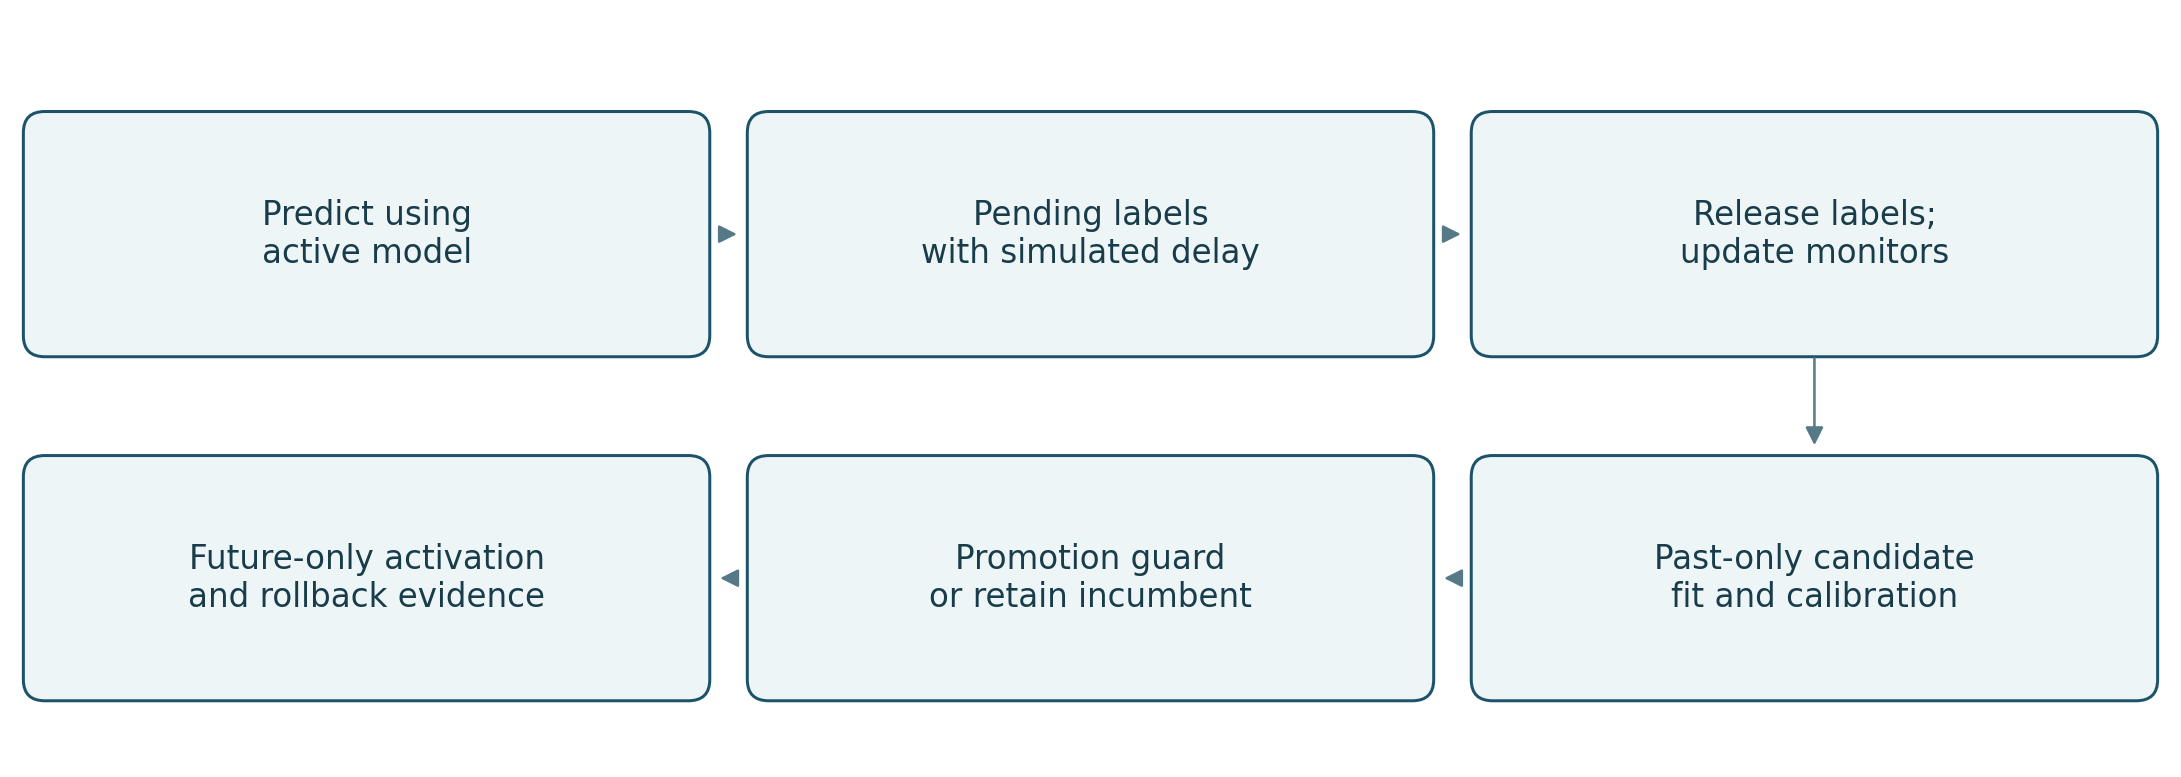
\includegraphics[width=\columnwidth]{../figures/adaptive_lifecycle.png}\caption{Future-only adaptive lifecycle. Labels are simulated as available according to the archived protocol; historical predictions are never revised by later candidates.}\label{fig:adaptive}\end{figure}
